\section{Computation} \label{sec:comp}
Simply deriving the equations for the PDF is not enough.
The many body nature of the PDF equation make analytical solution of the structure from the PDF impossible.
Thus, the PDF must be computed from a structural candidates and compared against experimental results to evaluate the reliability of the model.
These computations were implemented using high performance or high throughput computing methods (HPC or HTC) and Graphical Processing Units to provide quicker solutions.

\subsection{HPC and GPUs}
To properly solve the structure of materials the PDF will need to be computed many times and checked against experimental results.
This requires computation of the PDF, potentially over many atoms.
Calculating these PDFs requires a fast, highly parallelized, computational framework.
\subsubsection{GPUs and Parallelization}
\begin{figure}
    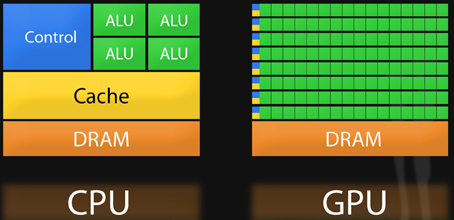
\includegraphics[width=\textwidth]{cpu_gpu}
    \caption[Comparison of the CPU and GPU chip architectures]{
    Comparison of the central processing unit (CPU) and GPU chip architectures from \cite{Chen2013}.
    The arithmetic logic unit (ALU) are the arithmetic logic units which perform the mathematical operations,
    the dynamic random-access memory (DRAM) holds most of the data, although it is slower to access,
    the Cache holds rapidly accessed data,
    and the Control controls the execution of software.
    Note the greater number of ALUs on the GPU, the comparatively smaller cache,
    and the allocation of caches and controls to entire rows of processors.}
    \label{fig:cpu_vs_gpu}
\end{figure}
Computing the PDF is an embarrassingly parallel problem.
The basic procedure is to calculate the reduced structure factor $F(Q)$ for each atom pair and momentum transfer vector, sum over all the atom pairs, and Fourier transform the structure to the PDF.
The first part of this procedure is perfectly parallelizable, as each atom pair is separate from the others.
The summation over all the atomic reduced structure factors can be parallelized via distributed summing.
Lastly the FFT can be parallelized using existing algorithms.

Graphical Processing Units (GPUs) are particularly well suited to the task of computing PDFs.
GPU chip architecture is designed to perform many task simultaneously by having potentially thousands of cores.
Figure \ref{fig:cpu_vs_gpu} show the comparison of CPU and GPU architectures.
As the figure shows the GPUs have a very different layout of computational processors (ALUs) and memory.
While each ALU is simpler on the GPU, requiring the instructions to be less demanding in terms of memory, there are many more of them.
The greater number of processors allows each atomic pairing to be placed on its own processor, so long as the math can be broken into simpler operations.
The equations are broken up on the GPUs into various pieces which correspond to the $\alpha, \beta, \uptau$ and $\Omega$ as shown in equations \ref{eq:alpha}-\ref{eq:omega} and sub-equations as needed.
For example, while $\beta$ is computed in one step, $\Omega$ requires the computation of the displacement array, then the distance array and finally the $\Omega$ array.
The exact breakdown of processes, how the problems are broken down and spread across the processor has been optimized for speed and reliability.

\subsubsection{Map from ij space to k space}
The above equations, although formally correct, are very inefficient. $F(Q)$ and its gradient are indexed over all the atoms twice, however there are symmetries that allow us to only compute over the atom pairs essentially mapping from an $n$x$n$ space, $ij$ space, to a $\frac{n(n-1)}{2}$ space, $k$ space.
For $F(Q)$ we apply the following mapping
\begin{figure}[!ht]
\begin{center}
\begin{tikzpicture}
    \node (E) at (0,0) {$E$};
    \node[right=of E] (F) {$E'$};
    \node[right=of F] (Z) {$Z$};
    \node[below=of F] (N) {$B'$};
    \node[below=of E] (M) {$B$};
    \draw[->] (E)--(F) node [midway,above] {$\psi$};
    \draw[->] (F)--(Z) node [midway,above] {$\Sigma$};
    \draw[->] (M)--(N) node [midway,below] {$\psi'$};
    \draw[->] (E)--(M) node [midway,left] {$\phi$};
    \draw[->] (N)--(Z) node [midway,left] {$\Sigma'$};
\end{tikzpicture}
\end{center}
\end{figure}
where $E$ denotes the atomic coordinates in $ij$ space, $E'$ denotes $F(Q)$ before the summation in $ij$ space, $B$ denotes the atomic pairs in $k$ space, $B'$ denotes $F(Q)$ in $k$ space, and $Z$ denotes the final summed $F(Q)$.  For the operators, $\phi$ denotes the mapping from $ij$ space to $k$ space $k = j + i * \frac{i - 1}{2}$, $\psi$ and $\psi'$ denote the $F(Q)$ operation in $ij$ and $k$ space, respectively. $\Sigma$ denotes the sum over all the atoms.

To properly define $\Sigma'$ we must establish whether $F(Q)$ is an even function.
We can accomplish this by examining each of the portions of $F(Q)$, $\alpha, \beta ,\uptau, \Omega$.
$\Omega$ is even, since $r_{ij}$ is the interatomic distance, which is the same despite a flip of indices, $Q$ does not depend on the atomic indices, and since $Qr_{ij}$ is even so is $\sin{Qr_{ij}}$.  Thus, $\Omega$ is even.  Providing similar analysis to $\uptau$ we can see that while $\vec{u}_{ij}$ is odd, so is the unit displacement vector between the two atoms, thus the two odds cancel out.
Intuitively this makes sense, since the $F(Q)$ equation is fundamentally interested in the interatomic distances which is even.  Thus, switching atom indices does not change $F(Q)$.
Due to the even nature of the $F(Q)$ operator the $\Sigma'$ operator sums over all the atom pairs, and multiplies by two to reflect the double counting of the $\Sigma$ operator.

For the gradient a similar mapping is used:
\begin{figure}[h!]
\begin{center}
  \begin{tikzpicture}
    \node (E) at (0,0) {$E$};
    \node[right=of E] (F) {$E'$};
    \node[right=of F] (Z) {$Z$};
    \node[below=of F] (N) {$B'$};
    \node[below=of E] (M) {$B$};
    \draw[->] (E)--(F) node [midway,above] {$\psi$};
    \draw[->] (F)--(Z) node [midway,above] {$\Sigma$};
    \draw[->] (M)--(N) node [midway,below] {$\psi'$};
    \draw[->] (E)--(M) node [midway,left] {$\phi$};
    \draw[->] (N)--(Z) node [midway,left] {$\tilde{\phi}\Sigma$};
\end{tikzpicture}
\end{center}
\end{figure}

In this mapping, however, we use the $\tilde{\phi}\Sigma$ operator.  This operator simultaneously performs a reverse mapping from $k$ to $ij$ space, and a summation with the correct symmetry.  In this case the $\psi$ and $\psi'$ operators, which denote the $\grad{F(Q)}$ operator in $ij$ and $k$ space, are antisymmetric.  Intuitively this makes sense as an extension of Newton's Second Law, since each particle's interaction is felt oppositely by its partner.
\subsubsection{GPU Memory Allocation}
While GPUs are very fast computational engines they tend to be memory bound.
While a gradient array for a 10nm Au nanoparticle, consisting of 31,000 atoms and half a billion unique distances, occupies 1.5 TB of memory a single GPU's RAM allotment varies from 4GB on a NVIDIA GTX970 to 24 GB on a NVIDIA Tesla K80.
Thus, it is important to determine exactly how many atoms can fit on a GPU of arbitrary size as a function of the number of atoms and the $Q$ range.
The memory required per array is:
\begin{eqnarray}
    q [=] 3n\\
    d [=] 3k\\
    r [=] k\\
    scatter [=] nQ\\
    normalization [=] kQ\\
    \Omega [=] kQ\\
    F_{k}(Q) [=] kQ\\
    Sum [=] kQ\\
    Sum2 [=] kQ\\
    F(Q) [=] Q
\end{eqnarray}
where $n$ is the number of atoms, $k$ is the number of unique distances, $Q$ is the scatter vector, and the $[=]$ operator denote the number of single precision floating point values in memory.
Each of the above arrays are used in the computation and thus must be able to be held in memory.
Thus the number of atom pairs that can fit on a GPU with $am$ bytes of available memory is:
\begin{equation}
    k_{per GPU} = \frac{1}{16 Q + 16} \left(- 4 Q n - 4 Q + am - 12 n\right)
\end{equation}
If ADPs are included in the calculation, then the following arrays are also added to the memory allocation:
\begin{eqnarray}
    adps = 3n\\
    \sigma = k\\
    \uptau = kQ
\end{eqnarray}
Thus the pair allotment is:
\begin{equation}
    k_{per GPU} = \frac{- 4 Q n - 4 Q + am - 24 n}{20 Q + 20}
\end{equation}

For the Gradient we need to calculate $F(Q)$ and its gradient, so the total memory overhead is equal to the previously mentioned arrays plus:
\begin{eqnarray}
    \grad{\Omega} = 3kQ \\
    \grad{F_{k}(Q)} = 3kQ \\
    \grad{F_{n}(Q)} = 3nQ
\end{eqnarray}
Thus the gradient allotment is:
\begin{equation}
    \grad{k_{per GPU}} = \frac{- 16 Q n + am - 12 n}{32 Q + 16}
\end{equation}
For the gradient with ADPs the ADP gradient array is:
\begin{equation}
    \grad{\uptau} = 3kQ
\end{equation}
Thus the allocation is:
\begin{equation}
    \grad{k_{per GPU}} = \frac{ - 16 Q n + am - 24 n}{48 Q + 20}
\end{equation}
These equations were solved by sympy as their validity is very important to the overall reliability of the software.
If the GPU is over allocated then the system may crash or return meaningless results.

\subsection{Speed and Scaling of PDF Computation}
To understand exactly how much the GPUs speed up the computation of $F(Q)$ and the PDF a series of time studies were run Au nanoparticles of varying size.
Figure \ref{fig:speed} shows the results of these time studies. CPU and GPU calculations were carried out on an Intel i7-4820K $@$3.70GHz Quad-Core and one NVIDIA GTX970s, respectively.
\begin{figure}
    \foreach \n in {fq_log, speed_log}{
        \subfloat[]{\includegraphics[width=.5\textwidth]{\n}}
        }
    \caption[Speed comparison of CPU and GPU implementations]{Speed comparison of CPU and GPU implementations.
    a) shows the time to compute the $F(Q)$ by itself.
    b) shows the time to compute the Rw based energy for Au NPs of various sizes, which includes computing $F(Q)$, its FFT, and the $Rw.$}
    \label{fig:speed}
\end{figure}
The $F(Q)$ computations show a 100x to 10x speedup using the GPUs over the CPUs.
Additionally, the $\grad{F(Q)}$ and $F(Q)$ computations seem to have similar computation time and scaling relationships on the GPU.
This implies that the two processes may have similar bottlenecks, most likely in the $F(Q)$ computation workflow.
This relationship is similarly preserved, although to a lesser extent, in the CPU scaling.

Interestingly, the tight run time relationship between $F(Q)$ and its gradient are not preserved in the $Rw$ based force calculations.
While the energy calculations are very similar to the $F(Q)$ calculations in terms of run time, the GPU and CPU force calculations are much closer, with the GPU calculations being much slower.
This is due to the force bottleneck being the $3n$ FFT operations which must be performed on the $\grad{F(Q)}$ array to produce the $\grad{\text{PDF}}$ array.
While the GPU is leveraged to perform the FFT, the data must be loaded off the GPU and back on, causing a potential slowdown.
Larger systems of atoms were not tried as the CPU computation quickly becomes very slow.
Even higher GPU  speedup is expected on more advanced GPUs like the NVIDIA Tesla series.